\begin{figure*}[t]
\centering
\noindent\textbf{(a) T04: resolving an infeasible reference initialization}\par\vspace{3pt}
\begin{minipage}[t]{0.225\textwidth}
\centering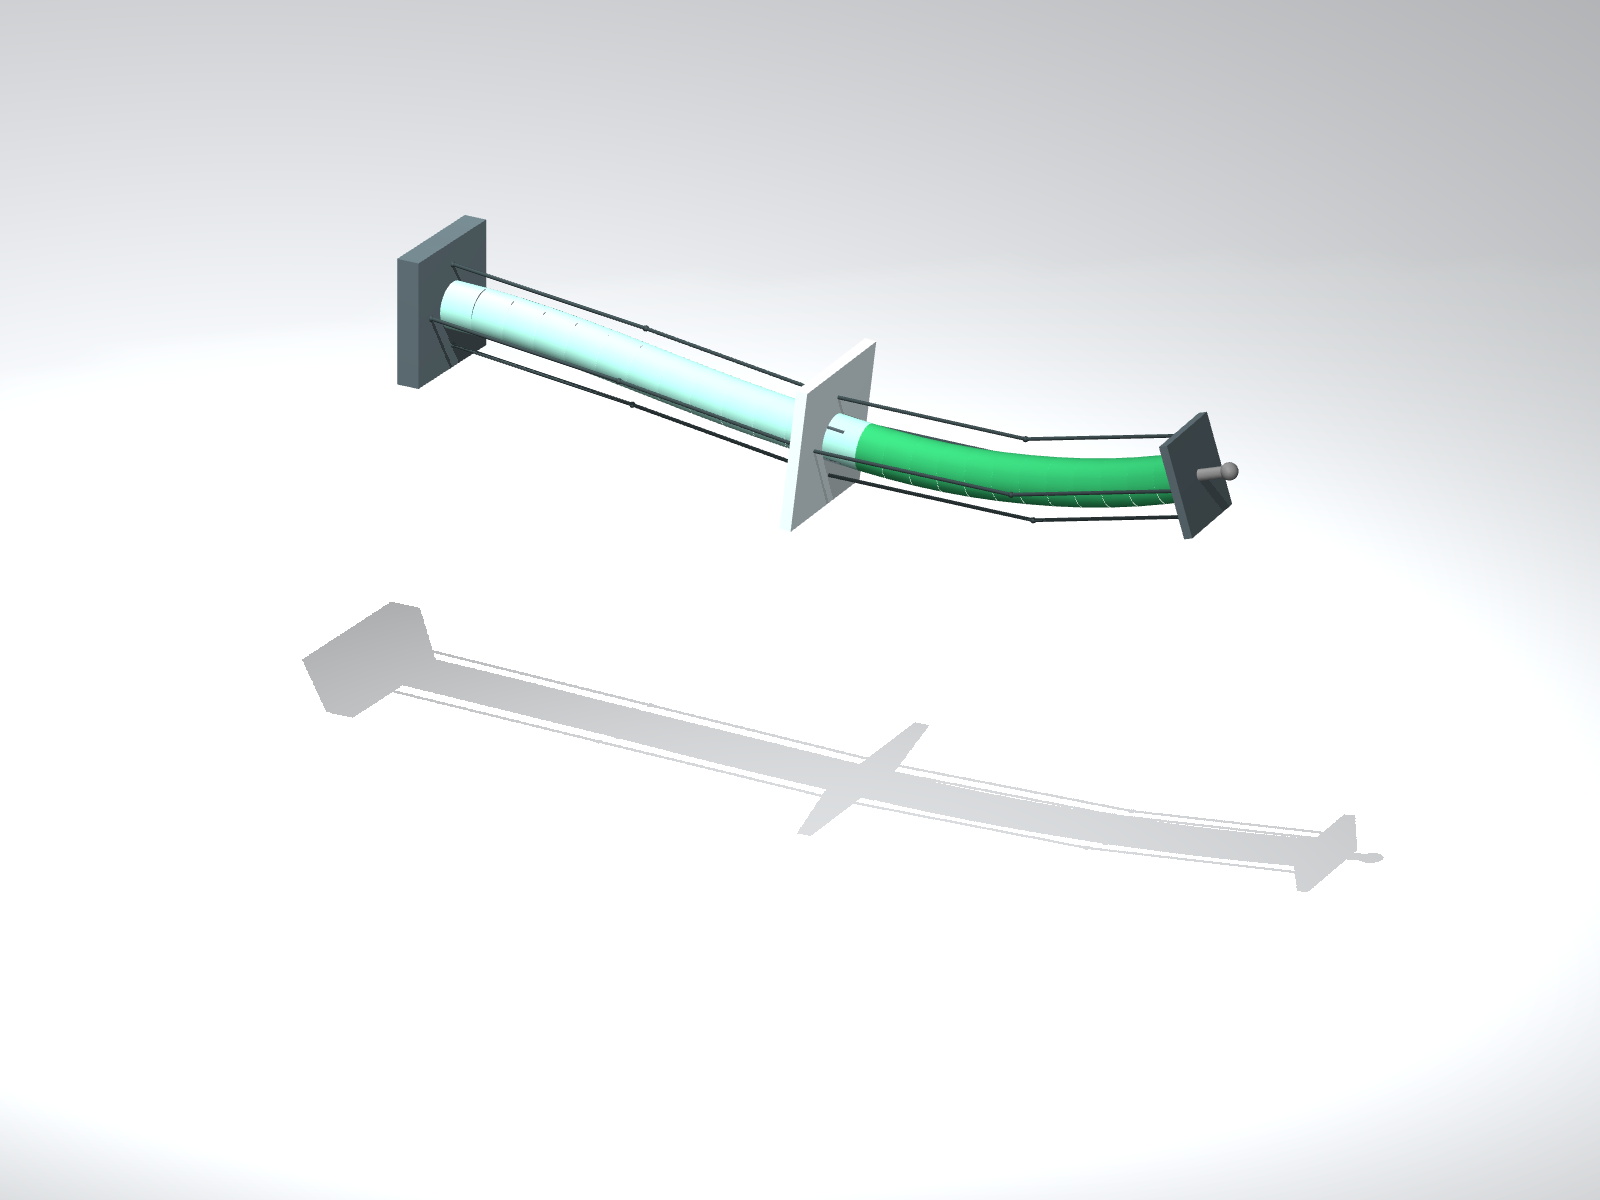
\includegraphics[width=\linewidth]{figures/native/t04_earlier_route.png}
\par\small Earlier native execution
\end{minipage}\hfill
\begin{minipage}[t]{0.225\textwidth}
\centering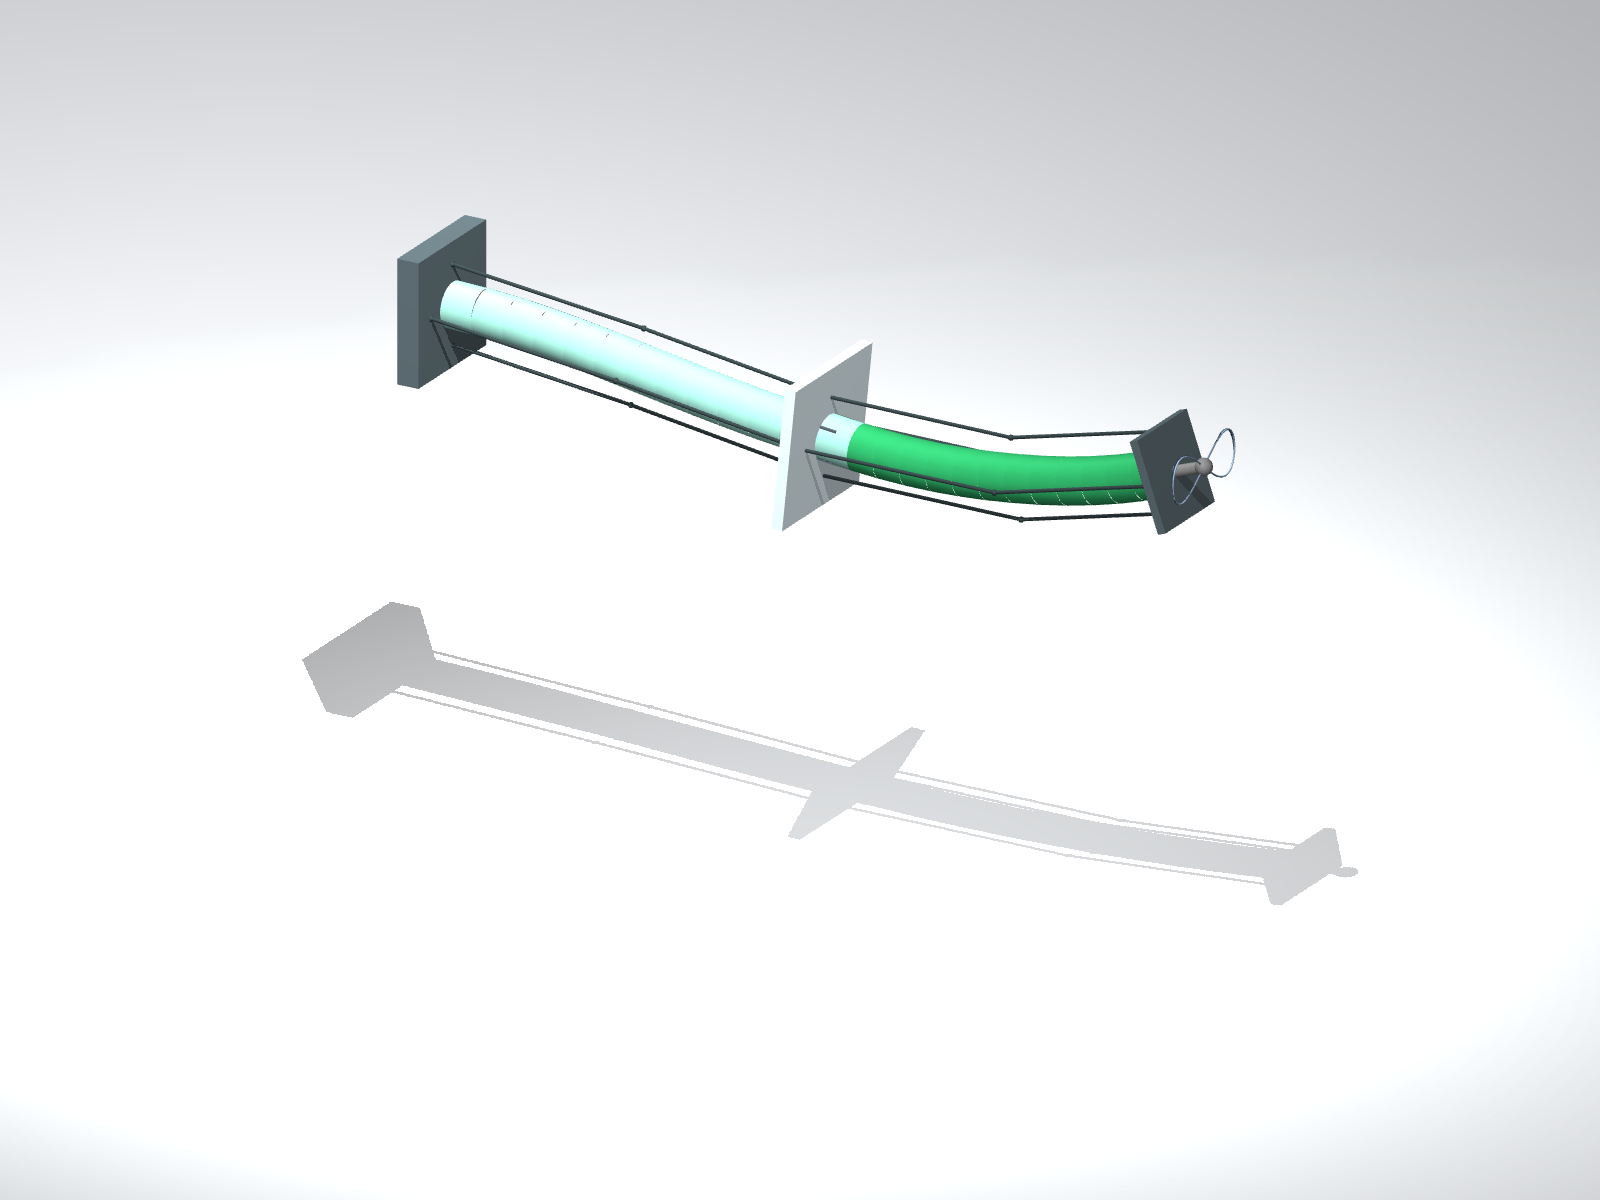
\includegraphics[width=\linewidth]{figures/native/t04_final.png}
\par\small Final execution
\end{minipage}\hfill
\begin{minipage}[t]{0.53\textwidth}
\centering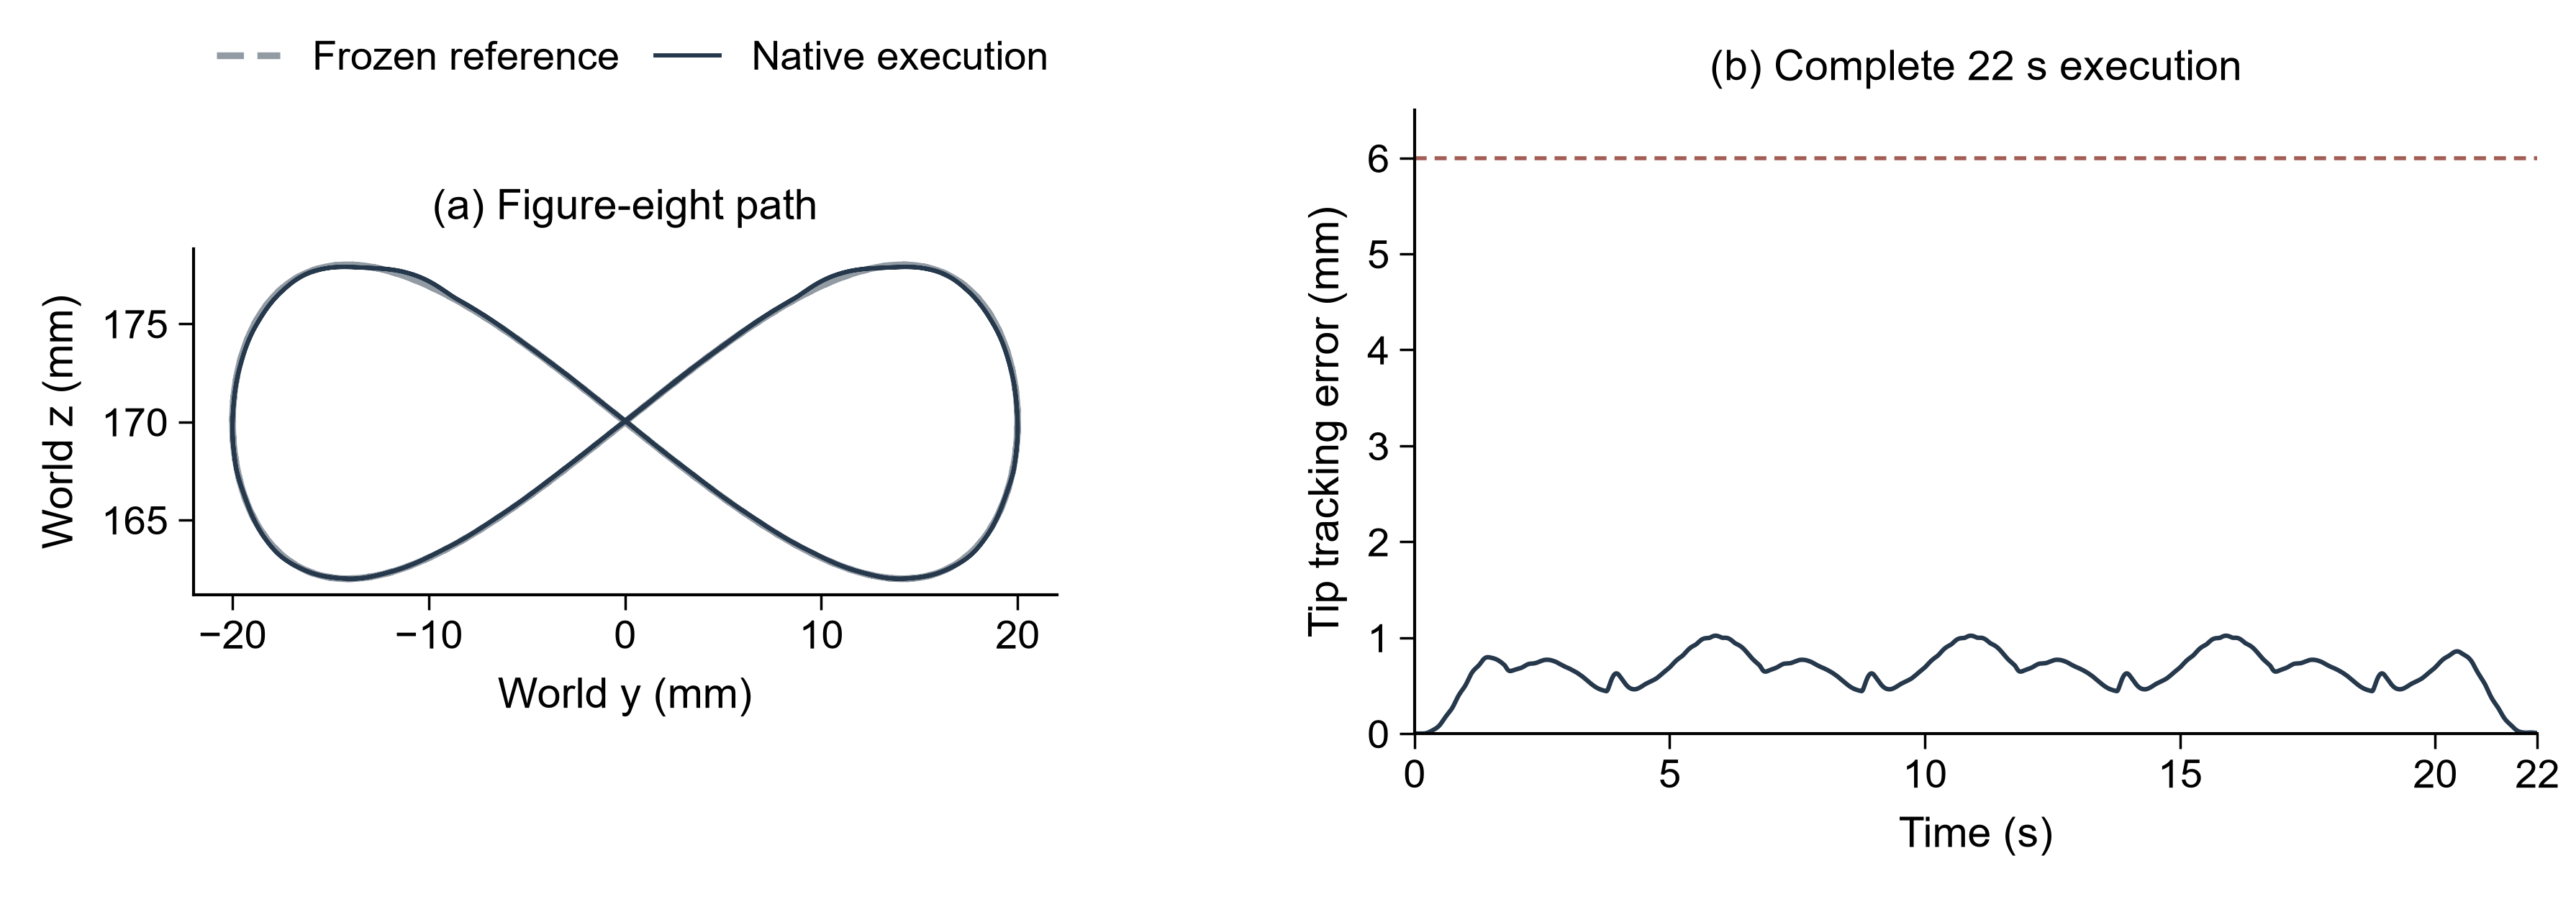
\includegraphics[width=\linewidth]{figures/native/t04_tracking.png}
\par\small Full two-cycle reference and tracking error
\end{minipage}
\par\vspace{3pt}
\noindent\small\textcolor{TraceNavy}{\textbf{Agent output:}}
\emph{The all-4 N initialization caused an inadmissible native optimizer trial.}
\quad\textcolor{TraceTeal}{\textbf{Action:}}
Restart from the time-zero equilibrium, shift boundary tensions from 0.20 to 0.21 N, and construct an 89-point reference bank.
\quad\textbf{Result:} 22 s; RMSE 0.688 mm; maximum error 1.021 mm.
\par\vspace{8pt}
\noindent\textbf{(b) T10: changing the controller while retaining the morphology}\par\vspace{3pt}
\begin{minipage}[t]{0.32\textwidth}
\centering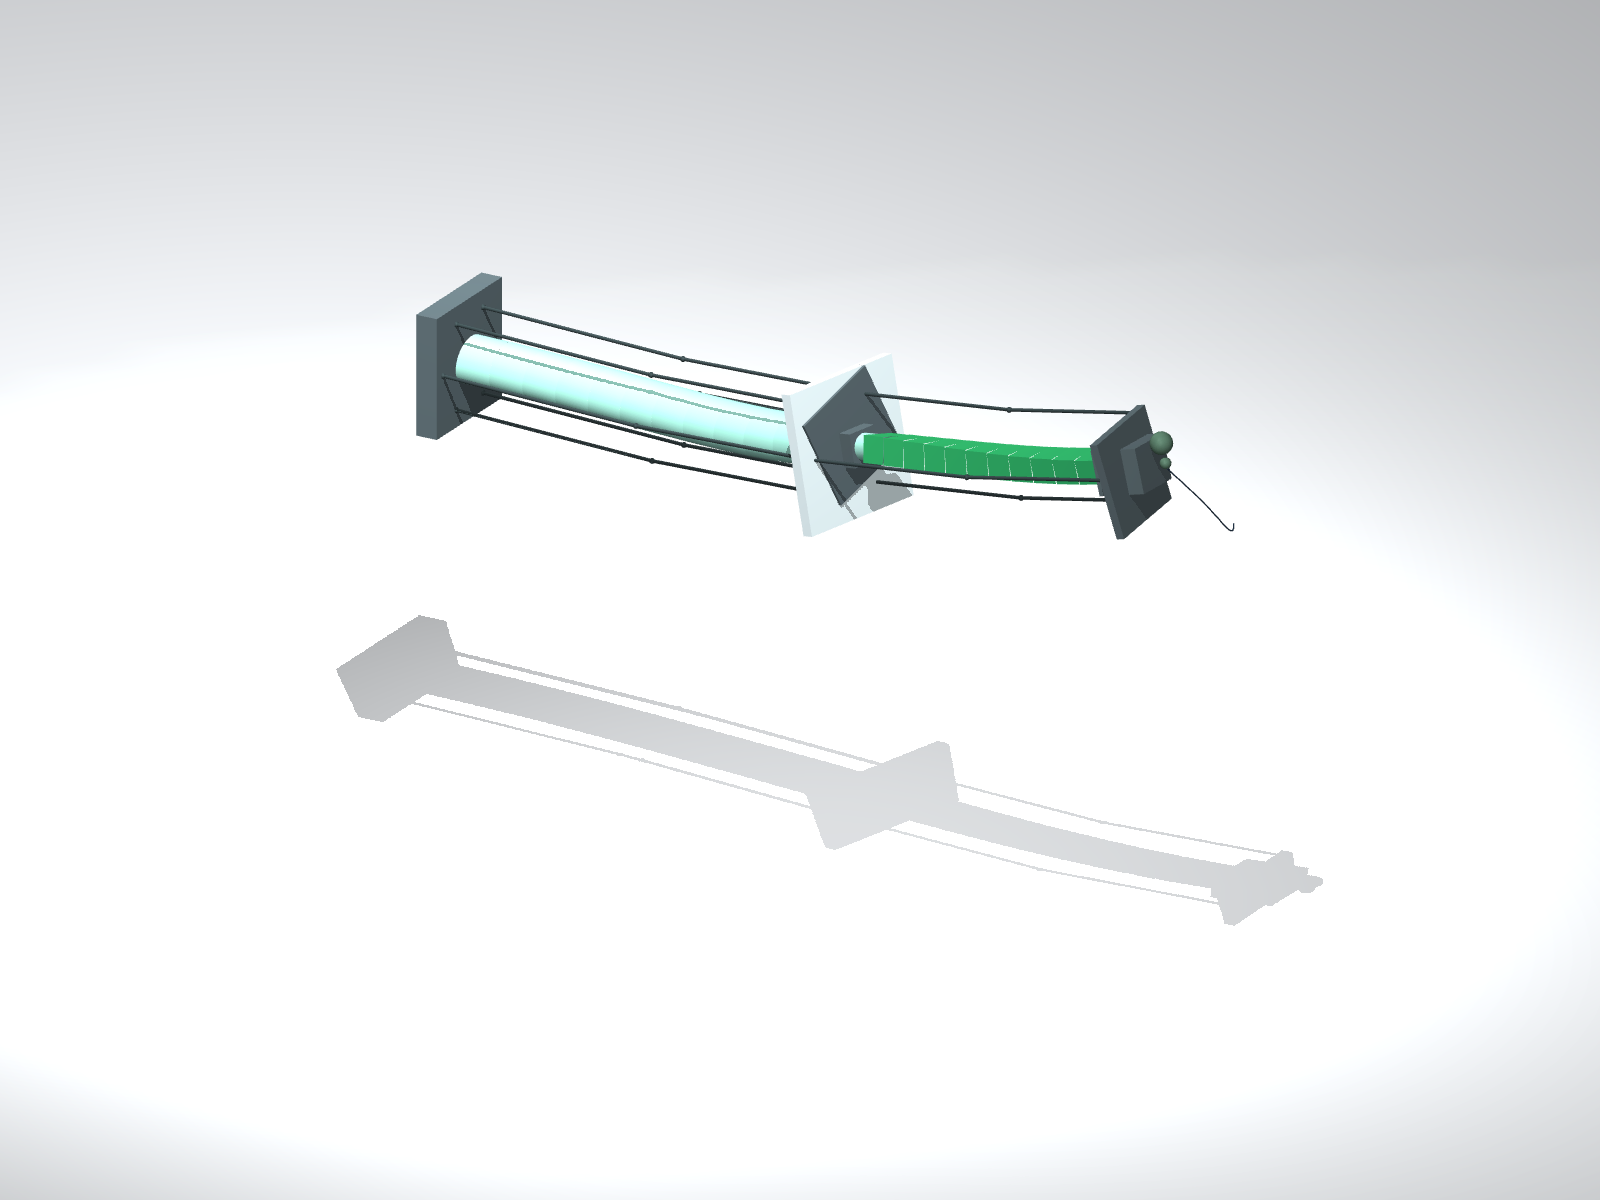
\includegraphics[width=\linewidth]{figures/native/t10_preimpact.png}
\par\small Pre-impact
\end{minipage}\hfill
\begin{minipage}[t]{0.32\textwidth}
\centering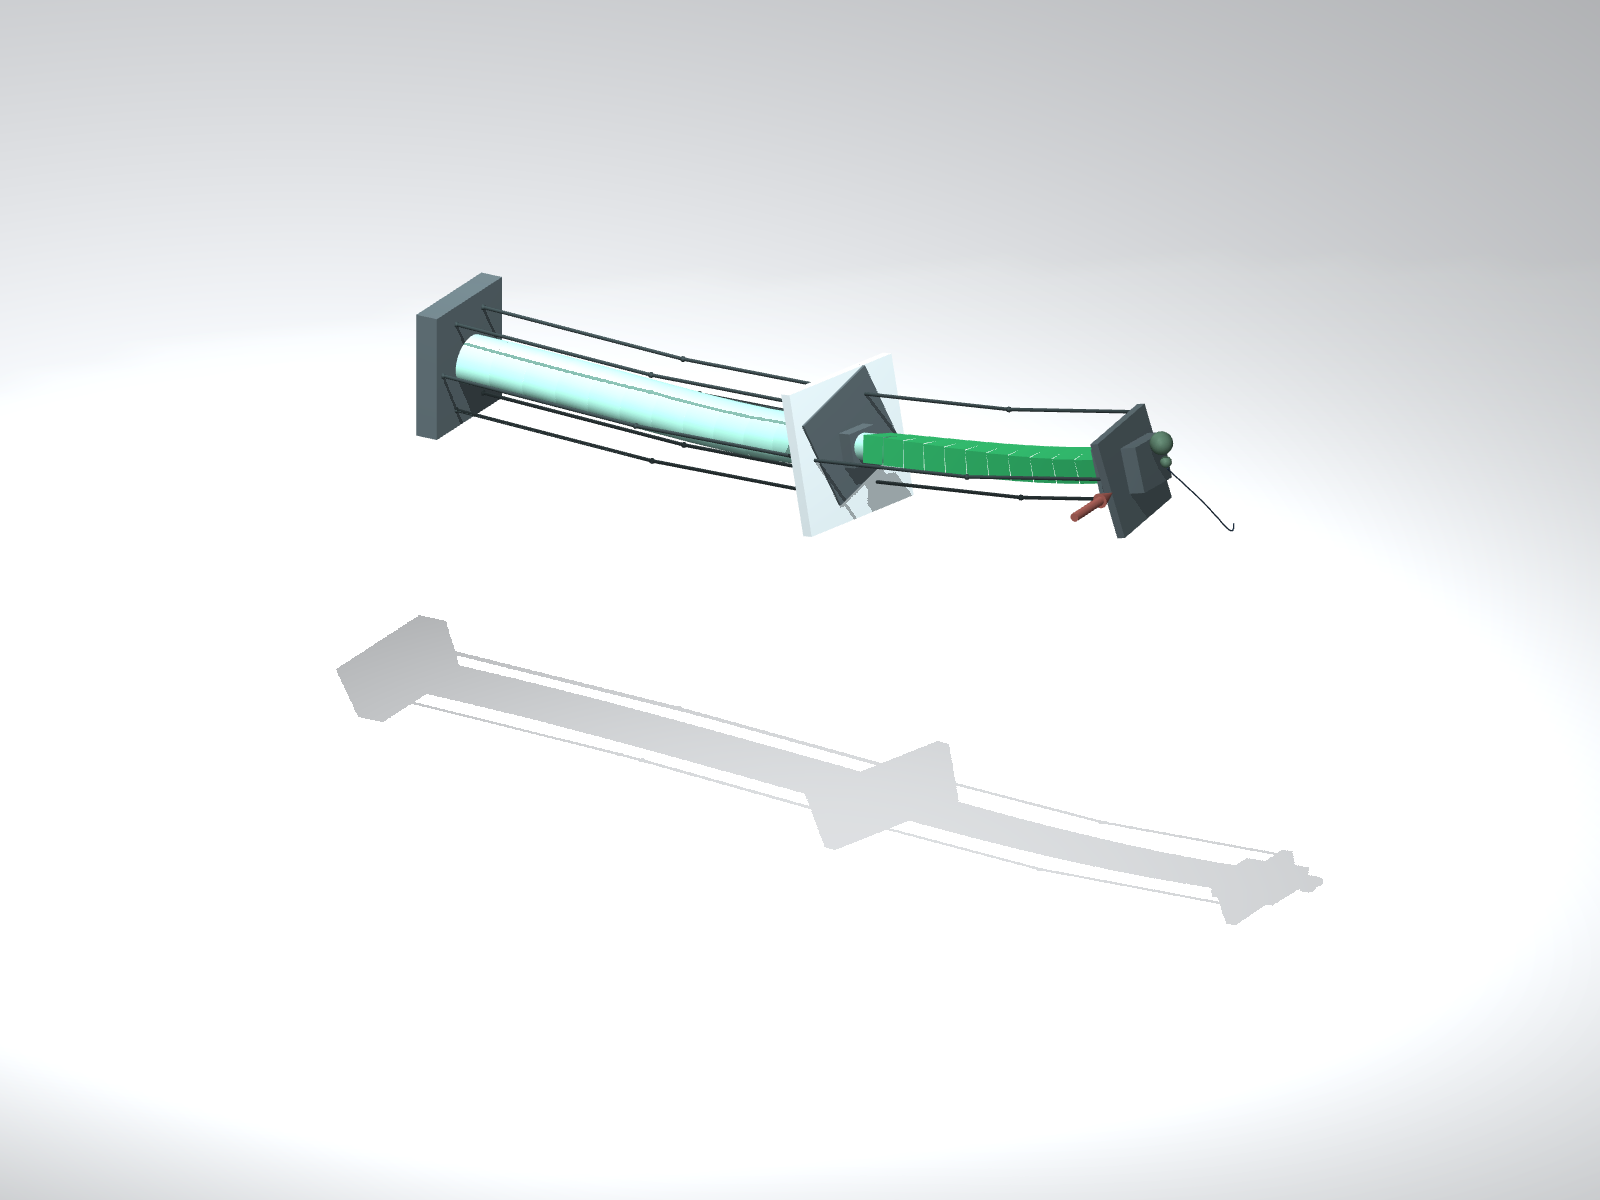
\includegraphics[width=\linewidth]{figures/native/t10_impact.png}
\par\small Disturbance
\end{minipage}\hfill
\begin{minipage}[t]{0.32\textwidth}
\centering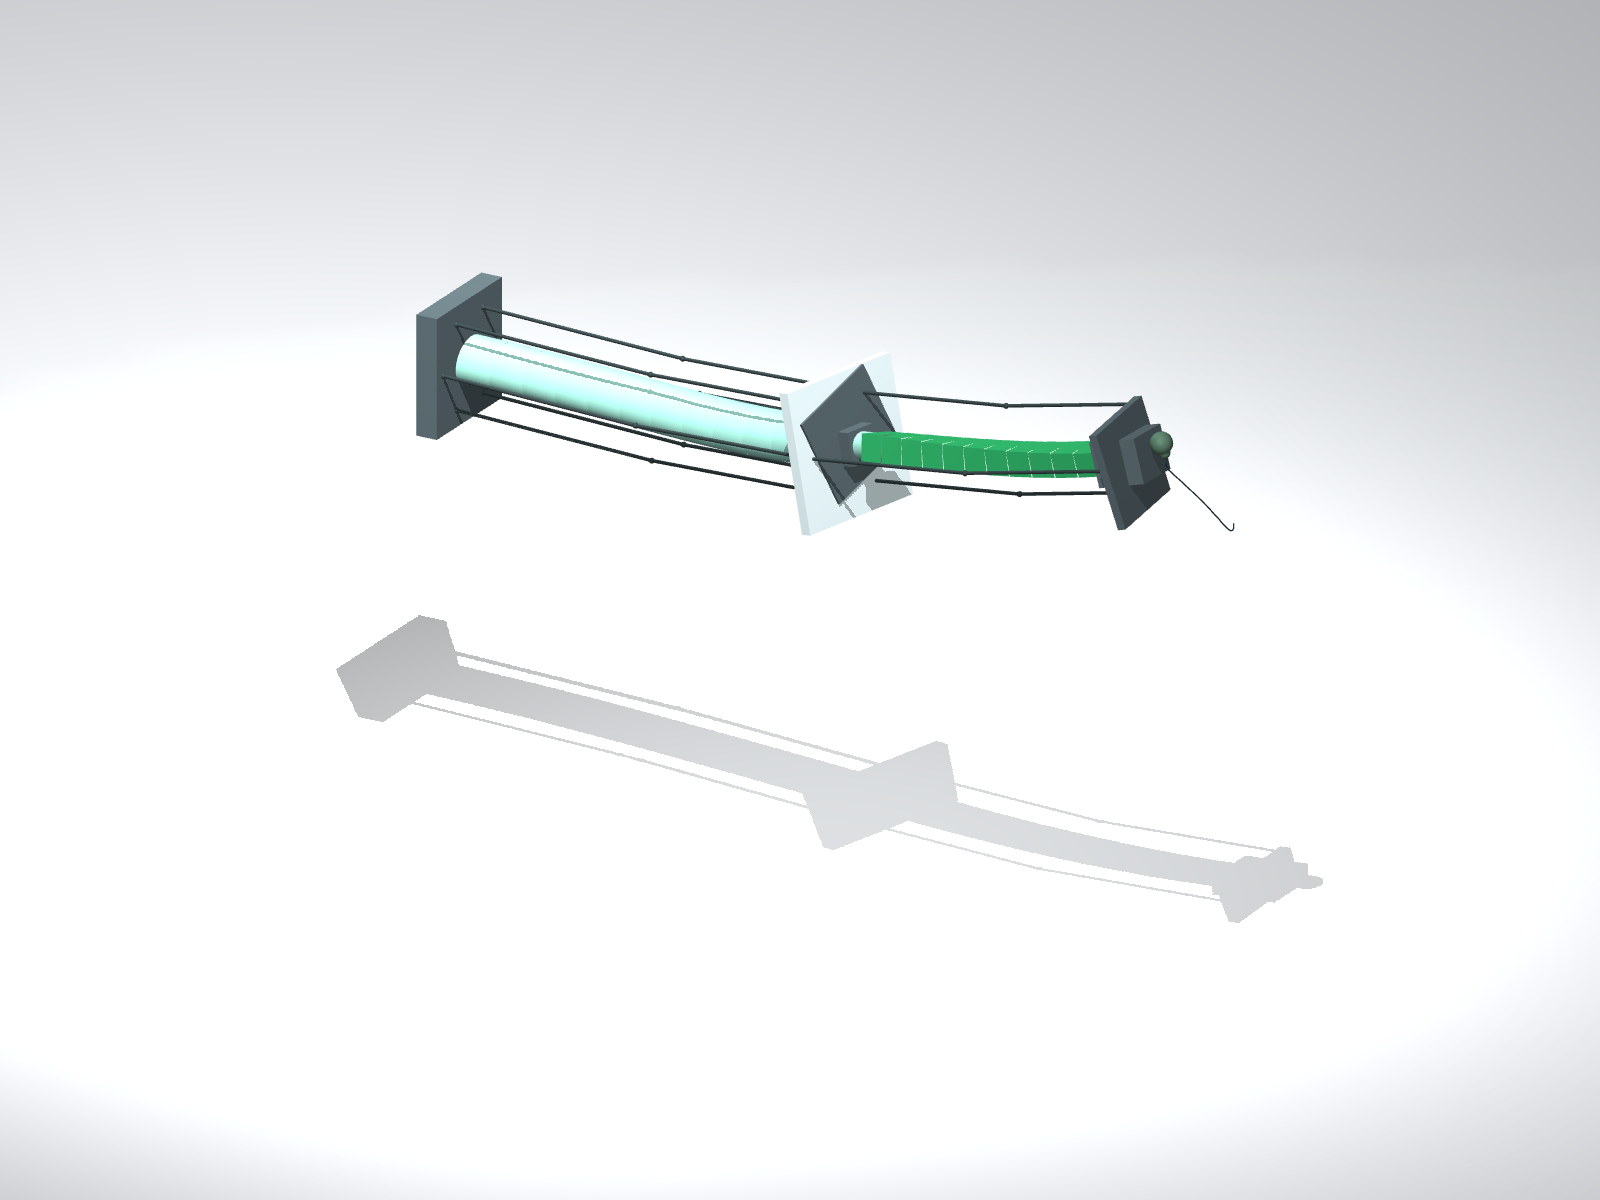
\includegraphics[width=\linewidth]{figures/native/t10_final_hold.png}
\par\small Recovered hold
\end{minipage}
\par\vspace{3pt}
\noindent\small\textcolor{TraceNavy}{\textbf{Agent diagnosis:}}
GVS/NMPC trials leave holding and tendon-limit conflicts.
\quad\textcolor{TraceTeal}{\textbf{Action:}}
Use a native tangent model, discrete LQR and bounded tension allocation.
\quad\textbf{Result:}
The common feedback recipe passes 3/3 required cases; both frozen-input controls fail.
\par\vspace{3pt}
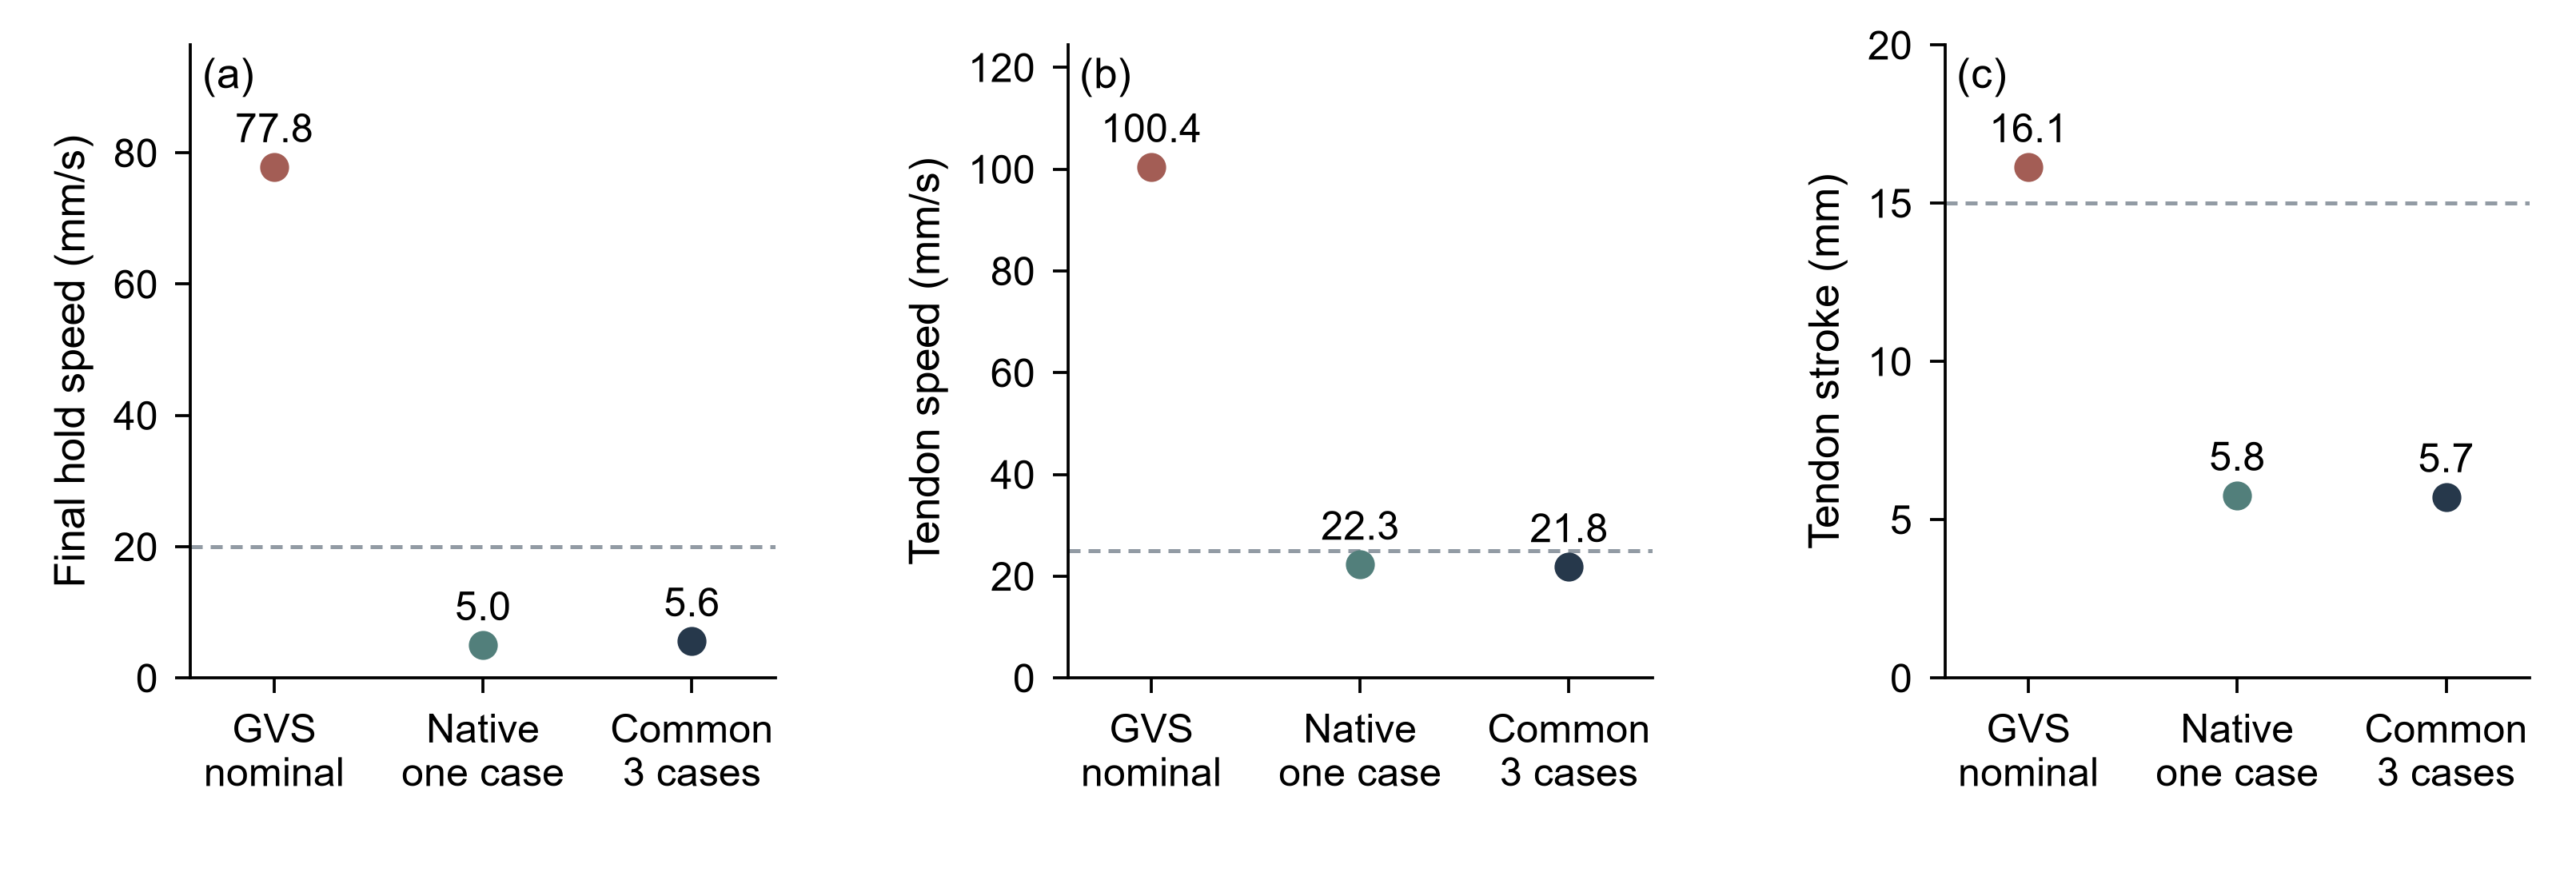
\includegraphics[width=0.78\textwidth]{figures/native/t10_control_comparison.png}
\caption{Representative research traces combining agent decisions, executed actions, native robot states and quantitative validation. T04 adapts reference-bank construction before tracking the complete figure-eight; T10 changes the control route on a fixed morphology.}
\label{fig:research-trajectory}
\end{figure*}
